%\documentclass[aspectratio=169]
\documentclass[aspectratio=169,xcolor=dvipsnames]{beamer}
%\usetheme{Copenhagen}
\usetheme{boxes}
\setbeamertemplate{navigation symbols}{}
%\setbeamertemplate{footline}[frame number]
\setbeamertemplate{footline}{
	\hfill%
	\usebeamercolor[fg]{page number in head/foot}%
	\usebeamerfont{page number in head/foot}%
	\setbeamertemplate{page number in head/foot}[framenumber]%
	\usebeamertemplate*{page number in head/foot}\kern1em\vskip2pt%
}
%\setbeamertemplate{footline}{}
\usecolortheme{dove}   %[named=black]

\usepackage[utf8]{inputenc}

\usepackage{graphicx}         
\graphicspath{ {./Pictures/} }
\usepackage{amsmath}
\usepackage{amsfonts}
\usepackage{amssymb}
\usepackage{amsthm}
\usepackage{mathtools}
\usepackage{commath}
\usepackage{multimedia}
\usepackage{subcaption}
\usepackage{media9}
\addmediapath{Animations/}
\newcommand{\Sta}{y}
\newcommand{\Adj}{p}
\newcommand{\Con}{u}
\begin{document}

\title[]{DDFT for Molecular and Colloidal Fluids:\\
A microscopic approach to fluid mechanics}
\author[]{A. J. Archer}
\institute[]{Loughborough University}
\date{Published on 7th January 2009, \\ The Journal of Chemical Physics}

\begin{frame}
\titlepage
\end{frame}
 
 

\begin{frame}
	\frametitle{What we're doing today}
	
	\begin{align*}
	\frac{d \mathbf{r}_i}{dt} &= \frac{\mathbf{p}_i}{m}\\
	\frac{d \mathbf{p}_i}{dt} &= - \gamma \mathbf{p}_i + \mathbf{X}_i(\mathbf{r}_i) + \mathbf{G}_i(t) \qquad \quad
	\end{align*}
	\vspace{-0.5cm}
	\begin{figure}
		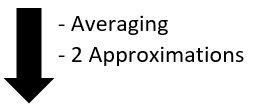
\includegraphics[width=3cm]{Arrow.png}
	\end{figure}
    \vspace{-0.3cm}
	\begin{align*}
	&\frac{\partial \rho}{\partial t} + \nabla \cdot \left(\rho \mathbf{v}\right) = 0 \\
	&\frac{\partial \mathbf{v}}{\partial t} + \mathbf{v} \cdot \left(\nabla \mathbf{v}\right) + \gamma \mathbf{v} = - \frac{1}{m}  \nabla \frac{\delta {F}[\rho]}{\delta \rho}
	\end{align*}
+ Bonus Material (time permitting)	
\end{frame}
\begin{frame}
	\frametitle{Part 1: From the microscopic equations to the N-body PDE}
	
	\begin{align*}
	\frac{d \mathbf{r}_i}{dt} &= \frac{\mathbf{p}_i}{m}\\
	\frac{d \mathbf{p}_i}{dt} &= - \gamma \mathbf{p}_i + \mathbf{X}_i(\mathbf{r}_i) + \mathbf{G}_i(t) \qquad \quad
	\end{align*}
	\vspace{-0.5cm}
	\begin{figure}
		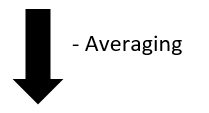
\includegraphics[width=3cm]{Arrow2.png}
	\end{figure}
	\vspace{-0.3cm}
	\begin{align*}
	\partial_t f^N = &- \frac{1}{m} \sum_{i=1}^N \mathbf{p}_i \cdot \nabla_{\mathbf{r}_i} f^N + \gamma \sum_{i = 1}^N \nabla_{\mathbf{p}_i}
	\cdot \mathbf{p}_i f^N - \sum_{i=1}^N \mathbf{X}_i \cdot \nabla_{\mathbf{p}_i}f^N + \gamma m k_BT \sum_{i=1}^N \nabla^2_{\mathbf{p}_i}f^N	
	\end{align*}

\end{frame}
\begin{frame}
	\frametitle{Part 2: From the N-body PDE to the one-body equations}
	\begin{align*}
	\partial_t f^N = &- \frac{1}{m} \sum_{i=1}^N \mathbf{p}_i \cdot \nabla_{\mathbf{r}_i} f^N + \gamma \sum_{i = 1}^N \nabla_{\mathbf{p}_i}
	\cdot \mathbf{p}_i f^N - \sum_{i=1}^N \mathbf{X}_i \cdot \nabla_{\mathbf{p}_i}f^N + \gamma m k_BT \sum_{i=1}^N \nabla^2_{\mathbf{p}_i}f^N	
	\end{align*}
	\vspace{-0.2cm}
	\begin{figure}
		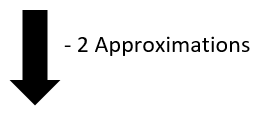
\includegraphics[width=4cm]{Arrow3.png}
	\end{figure}
	\vspace{-0.3cm}
	\begin{align*}
	&\frac{\partial \rho}{\partial t} + \nabla \cdot \left(\rho \mathbf{v}\right) = 0 \\
	&\frac{\partial \mathbf{v}}{\partial t} + \mathbf{v} \cdot \left(\nabla \mathbf{v}\right) + \gamma \mathbf{v} = - \frac{1}{m} \nabla \frac{\delta {F}[\rho]}{\delta \rho}
	\end{align*}
\end{frame}
\begin{frame}
	\centering
	\textbf{ \huge Part 1}
\end{frame}
\begin{frame}
	\frametitle{Part 1: From the microscopic equations to the N-body PDE}
	
	\begin{align*}
	\frac{d \mathbf{r}_i}{dt} &= \frac{\mathbf{p}_i}{m}\\
	\frac{d \mathbf{p}_i}{dt} &= - \gamma \mathbf{p}_i + \mathbf{X}_i(\mathbf{r}_i) + \mathbf{G}_i(t) \qquad \quad
	\end{align*}
	\vspace{-0.5cm}
	\begin{figure}
		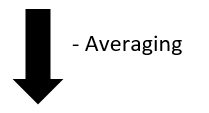
\includegraphics[width=3cm]{Arrow2.png}
	\end{figure}
	\vspace{-0.3cm}
	\begin{align*}
	\partial_t f^N = &- \frac{1}{m} \sum_{i=1}^N \mathbf{p}_i \cdot \nabla_{\mathbf{r}_i} f^N + \gamma \sum_{i = 1}^N \nabla_{\mathbf{p}_i}
	\cdot \mathbf{p}_i f^N - \sum_{i=1}^N \mathbf{X}_i \cdot \nabla_{\mathbf{p}_i}f^N + \gamma m k_BT \sum_{i=1}^N \nabla^2_{\mathbf{p}_i}f^N	
	\end{align*}
	
\end{frame}
\begin{frame}
	\frametitle{Part 1: From the microscopic equations to the N-body PDE}
	\textbf{The microscopic equations (1)}
	\vspace{0.2cm}
    \begin{align*}
	\frac{d \mathbf{r}_i}{dt} &= \frac{\mathbf{p}_i}{m}\\
	\frac{d \mathbf{p}_i}{dt} &= - \gamma \mathbf{p}_i + \mathbf{X}_i(\mathbf{r}_i) + \mathbf{G}_i(t) \qquad \quad\\
	\\
	\\
	\mathbf{G}_i(t) &\qquad \text{stochastic white noise term}\\
	\mathbf{X}_i(\mathbf{r}_i) &= - \nabla_{\mathbf{r}_i} V(\mathbf{r}^N,t) \qquad \text{sum of forces on particle } i\\
        &= - \nabla_{\mathbf{r}_i} \bigg(\sum_i V^{ext}(\mathbf{r}_i,t) + \frac{1}{2} \sum_{i,j} v_2(\mathbf{r}_i, \mathbf{r}_j)+ \frac{1}{6} \sum_{i,j,k} v_3 (\mathbf{r}_i, \mathbf{r}_j, \mathbf{r}_k) + ... \bigg)
	\end{align*}
\end{frame}

\begin{frame}
	\frametitle{Part 1: From the microscopic equations to the N-body PDE}
	\textbf{The hand-wavy derivation} \\(see MAC-MIGs modelling course, Lecture 3)
	\vspace{0.2cm}
	\begin{enumerate}
		\item Define $\psi^N(\mathbf{r}^N, \mathbf{p}^N, t)$, where $\mathbf{r}^N = \left\{\mathbf{r}_1, \mathbf{r}_2,..., \mathbf{r}_N\right\}$ and $\mathbf{p}^N = \left\{\mathbf{p}_1, \mathbf{p}_2,..., \mathbf{p}_N\right\}$
		\item Apply It\^{o}'s Lemma to $\psi^N$, using the microscopic equations, to get:
		\begin{align*}
		d\psi^N = {\mathcal{L} \psi^N} dt + B dW
		\end{align*} 
		\item Define average $\langle \psi^N\rangle$ and apply to the process $ d \psi^N$:
		\begin{align*}
		\langle d \psi^N \rangle = \langle  {\mathcal{L} \psi^N} dt\rangle + \langle B dW \rangle = \langle  {\mathcal{L} \psi^N} dt\rangle + 0
		\end{align*}
		\item Average is integral against the probability distribution $f^N(\mathbf{r}^N, \mathbf{p}^N, t)$
		\begin{align*}
		 LHS = \langle \frac{d}{dt} \textcolor{blue}{\psi^N} \rangle &:= \int \int\frac{d}{dt} \textcolor{blue}{\psi^N} f^N d\mathbf{r}^N d\mathbf{p}^N\\
		 RHS = \langle \textcolor{blue}{\mathcal{L} \psi^N}\rangle &:= \int \int\textcolor{blue}{\mathcal{L} \psi^N} f^N d\mathbf{r}^N d\mathbf{p}^N
		\end{align*}
	\end{enumerate}

\end{frame}
\begin{frame}
	\frametitle{Part 1: From the microscopic equations to the N-body PDE}
	\textbf{The hand-wavy derivation, continued}
		\vspace{0.2cm}
	\begin{enumerate}
		\setcounter{enumi}{4}
		\item Integrate by parts to get derivatives in terms of $f^N$ instead of $\psi^N$
		\begin{align*}
		LHS = \int \int\frac{d}{dt} \psi^N f^N d\mathbf{r}^N d\mathbf{p}^N &= -\int \int \psi^N \textcolor{red}{\partial_t f^N} d\mathbf{r}^N d\mathbf{p}^N \\
		RHS = \int \int\mathcal{L} \psi^N f^N d\mathbf{r}^N d\mathbf{p}^N &= - \int \int \psi^N \ \textcolor{red}{\mathcal{L}^* f^N}\ d\mathbf{r}^N d\mathbf{p}^N
		\end{align*}
		\item Since this holds for all $\psi^N$\\
			\vspace{0.2cm}
		$\Rightarrow$  $\textcolor{red}{\partial_t f^N = \mathcal{L}^* f^N}$
	\end{enumerate}
	
\end{frame}

\begin{frame}
	\frametitle{Part 1: From the microscopic equations to the N-body PDE}
	\textbf{The N-body PDE for the distribution $f^N(\mathbf{r}^N, \mathbf{p}^N,t)$ (6)}
	\begin{align*}
    \textcolor{red}{\partial_t f^N = \mathcal{L}^* f^N }&= - \frac{1}{m} \sum_{i=1}^N \mathbf{p}_i \cdot \nabla_{\mathbf{r}_i} f^N\\
    &+ \gamma \sum_{i = 1}^N \nabla_{\mathbf{p}_i}
    \cdot \mathbf{p}_i f^N - \sum_{i=1}^N \mathbf{X}_i \cdot \nabla_{\mathbf{p}_i}f^N + \gamma m k_BT \sum_{i=1}^N \nabla^2_{\mathbf{p}_i}f^N	
	\end{align*}
	\textbf{Reminder: the microscopic equations (1)}
	\begin{align*}
	\frac{d \mathbf{r}_i}{dt} &= \frac{\mathbf{p}_i}{m}\\
	\frac{d \mathbf{p}_i}{dt} &= - \gamma \mathbf{p}_i + \mathbf{X}_i(\mathbf{r}_i) + \mathbf{G}_i(t) \qquad \quad
	\end{align*}
\end{frame}
\begin{frame}
	\frametitle{Part 1: From the microscopic equations to the N-body PDE}
	
	\begin{align*}
	\frac{d \mathbf{r}_i}{dt} &= \frac{\mathbf{p}_i}{m}\\
	\frac{d \mathbf{p}_i}{dt} &= - \gamma \mathbf{p}_i + \mathbf{X}_i(\mathbf{r}_i) + \mathbf{G}_i(t) \qquad \quad
	\end{align*}
	\vspace{-0.5cm}
	\begin{figure}
		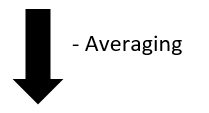
\includegraphics[width=3cm]{Arrow2.png}
	\end{figure}
	\vspace{-0.3cm}
	\begin{align*}
	\partial_t f^N = &- \frac{1}{m} \sum_{i=1}^N \mathbf{p}_i \cdot \nabla_{\mathbf{r}_i} f^N + \gamma \sum_{i = 1}^N \nabla_{\mathbf{p}_i}
	\cdot \mathbf{p}_i f^N - \sum_{i=1}^N \mathbf{X}_i \cdot \nabla_{\mathbf{p}_i}f^N + \gamma m k_BT \sum_{i=1}^N \nabla^2_{\mathbf{p}_i}f^N	
	\end{align*}
	
\end{frame}
\begin{frame}
	\centering
	\textbf{ \huge Part 2}
\end{frame}
\begin{frame}
	\frametitle{Part 2: From the N-body PDE to the one-body equations}
    \begin{align*}
	\partial_t f^N = &- \frac{1}{m} \sum_{i=1}^N \mathbf{p}_i \cdot \nabla_{\mathbf{r}_i} f^N + \gamma \sum_{i = 1}^N \nabla_{\mathbf{p}_i}
	\cdot \mathbf{p}_i f^N - \sum_{i=1}^N \mathbf{X}_i \cdot \nabla_{\mathbf{p}_i}f^N + \gamma m k_BT \sum_{i=1}^N \nabla^2_{\mathbf{p}_i}f^N	
	\end{align*}
		\vspace{-0.2cm}
	\begin{figure}
		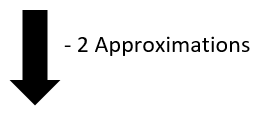
\includegraphics[width=4cm]{Arrow3.png}
	\end{figure}
	\vspace{-0.3cm}
	\begin{align*}
	&\frac{\partial \rho}{\partial t} + \nabla \cdot \left(\rho \mathbf{v}\right) = 0 \\
	&\frac{\partial \mathbf{v}}{\partial t} + \mathbf{v} \cdot \left(\nabla \mathbf{v}\right) + \gamma \mathbf{v} = - \frac{1}{m} \nabla \frac{\delta {F}[\rho]}{\delta \rho}
	\end{align*}
\end{frame}

\begin{frame}
	\frametitle{Part 2: From the N-body PDE to the one-body equations}
	1. Multiply (6) by $N$ and integrate over $\mathbf{r}^{N-1}, \ \mathbf{p}^{N-1}$
	\begin{align*}
	 \textcolor{red}{\int \int N }\partial_t f^N  \textcolor{red}{d \mathbf{r}^{N-1} d\mathbf{p}^{N-1}} = & \textcolor{red}{\int \int N} \bigg[ - \frac{1}{m} \sum_{i=1}^N \mathbf{p}_i \cdot \nabla_{\mathbf{r}_i} f^N + \gamma \sum_{i = 1}^N \nabla_{\mathbf{p}_i}
	\cdot \mathbf{p}_i f^N \\
	&- \sum_{i=1}^N \mathbf{X}_i \cdot \nabla_{\mathbf{p}_i}f^N + \gamma m k_BT \sum_{i=1}^N \nabla^2_{\mathbf{p}_i}f^N \bigg] \textcolor{red}{d \mathbf{r}^{N-1} d \mathbf{p}^{N-1}	}
	\end{align*}
	Define reduced distribution functions (7):
	\begin{align*}
	f^1(\mathbf{r}_1,\mathbf{p}_1,t) &= \ \ \ \ \ \ \  \ N \ \ \int \int f^N d\mathbf{r}^{N-1} d\mathbf{p}^{N-1}\\
	&...\\
	f^n(\mathbf{r}^n,\mathbf{p}^n,t) &= \frac{N!}{(N-n)!} \int \int f^N d\mathbf{r}^{N-n} d\mathbf{p}^{N-n}\\
	\end{align*}
\end{frame}
\begin{frame}
	\frametitle{Part 2: From the N-body PDE to the one-body equations}
	1. Multiply (6) by $N$ and integrate over $\mathbf{r}^{N-1}, \ \mathbf{p}^{N-1}$
	\begin{align*}
	\textcolor{blue}{\int \int N \partial_t f^N d \mathbf{r}^{N-1} d\mathbf{p}^{N-1}} = &\int \int N \bigg[ - \frac{1}{m} \sum_{i=1}^N \mathbf{p}_i \cdot \nabla_{\mathbf{r}_i} f^N + \gamma \sum_{i = 1}^N \nabla_{\mathbf{p}_i}
	\cdot \mathbf{p}_i f^N \\
	&- \sum_{i=1}^N \mathbf{X}_i \cdot \nabla_{\mathbf{p}_i}f^N + \gamma m k_BT \sum_{i=1}^N \nabla^2_{\mathbf{p}_i}f^N \bigg]d \mathbf{r}^{N-1} d \mathbf{p}^{N-1}	
	\end{align*}
	 Define reduced distribution functions (7):
	\begin{align*}
	f^1(\mathbf{r}_1,\mathbf{p}_1,t) &= \ \ \ \ \ \ \  \ N \ \ \int \int f^N d\mathbf{r}^{N-1} d\mathbf{p}^{N-1}\\
	&...\\
	f^n(\mathbf{r}^n,\mathbf{p}^n,t) &= \frac{N!}{(N-n)!} \int \int f^N d\mathbf{r}^{N-n} d\mathbf{p}^{N-n}\\
	\end{align*}
\end{frame}

\begin{frame}
	\frametitle{Part 2: From the N-body PDE to the one-body equations}
	Example:
	\begin{align*}
	 \textcolor{blue}{\int \int N \partial_t f^N d \mathbf{r}^{N-1} d\mathbf{p}^{N-1}} &= \partial_t N \int \int   f^N d \mathbf{r}^{N-1} d\mathbf{p}^{N-1} \\
	 &=  \partial_t f^1(\mathbf{r}_1,\mathbf{p}_1,t)
	 \end{align*}
	 where
	 \begin{align*}
	 f^1(\mathbf{r}_1,\mathbf{p}_1,t) &=  N \int \int f^N d\mathbf{r}^{N-1} d\mathbf{p}^{N-1}\\
	\end{align*}
\end{frame}
\begin{frame}
	\frametitle{Part 2: From the N-body PDE to the one-body equations}
	\begin{align*}
	\textcolor{blue}{\int \int N \partial_t f^N d \mathbf{r}^{N-1} d\mathbf{p}^{N-1}} = &\int \int N \bigg[ - \frac{1}{m} \sum_{i=1}^N \mathbf{p}_i \cdot \nabla_{\mathbf{r}_i} f^N + \gamma \sum_{i = 1}^N \nabla_{\mathbf{p}_i}
	\cdot \mathbf{p}_i f^N 
	- \sum_{i=1}^N \textcolor{ForestGreen}{\mathbf{X}_i} \cdot \nabla_{\mathbf{p}_i}f^N \\
	&+ \gamma m k_BT \sum_{i=1}^N \nabla^2_{\mathbf{p}_i}f^N \bigg]d \mathbf{r}^{N-1} d \mathbf{p}^{N-1}	
	\end{align*}
	\vspace{-0.2cm}
	where (1):
	\begin{align*}
	\textcolor{ForestGreen}{\mathbf{X}_i(\mathbf{r}_i) = - \nabla_{\mathbf{r}_i} \bigg(\sum_i V^{ext}(\mathbf{r}_i,t) + \frac{1}{2} \sum_{i,j} v_2(\mathbf{r}_i, \mathbf{r}_j)+ ... \bigg)}
	\end{align*}
	\vspace{-0.2cm}
    We get (8):
	\begin{align*}
	\textcolor{blue}{\partial_t f^1} &=- \frac{\mathbf{p}_1}{m} \cdot \nabla_{\mathbf{r}_1}f^1 + \gamma \nabla_{\mathbf{p}_1} \cdot \left(\mathbf{p}_1 f^1\right)
    + \textcolor{ForestGreen}{\nabla_{\mathbf{r}_1}V^{ext}(\mathbf{r}_1)} \cdot \nabla_{\mathbf{p}_1}f^1 \\
    &+ \gamma mk_bT \nabla^2_{\mathbf{p}_1} f^1 + \int \int \textcolor{ForestGreen}{\nabla_{\mathbf{r}_1}v_2(\mathbf{r}_1 - \mathbf{r}_2)} \cdot \nabla_{\mathbf{p}_1}f^2 d \mathbf{r}_2 d \mathbf{p}_2 + ...
	\end{align*}

\end{frame}
\begin{frame}
	\frametitle{Part 2: From the N-body PDE to the one-body equations}
	\vspace{0.5 cm}
	\textbf{Taking two momentum moments to give 2 equations:}\\
	2. First momentum moment: Integrate with respect to $\mathbf{p}_1$\\
	3. Second momentum moment: Multiply by $\frac{\mathbf{p}_1}{m}$, then integrate with respect to $\mathbf{p}_1$\\
	\vspace{1 cm}
	2. First momentum moment: Integrate with respect to $\mathbf{p}_1$:
\begin{align*}
\textcolor{red}{\int}{\partial_t f^1} \textcolor{red}{d \mathbf{p}_1}&= \textcolor{red}{\int \bigg[} - \frac{\mathbf{p}_1}{m} \cdot \nabla_{\mathbf{r}_1}f^1 + \gamma \nabla_{\mathbf{p}_1} \cdot \left(\mathbf{p}_1 f^1\right)
+ {\nabla_{\mathbf{r}_1}V^{ext}(\mathbf{r}_1)} \cdot \nabla_{\mathbf{p}_1}f^1\\
&+ \gamma mk_bT \nabla^2_{\mathbf{p}_1} f^1 + \int \int {\nabla_{\mathbf{r}_1}v_2(\mathbf{r}_1 - \mathbf{r}_2)} \cdot \nabla_{\mathbf{p}_1}f^2 d \mathbf{r}_2 d \mathbf{p}_2 + ... \textcolor{red}{\bigg] d \mathbf{p}_1}
\end{align*}

	
	
\end{frame}


\begin{frame}
	\frametitle{Part 2: From the N-body PDE to the one-body equations}
	2. First momentum moment: Integrate with respect to $\mathbf{p}_1$
	\begin{align*}
	\textcolor{blue}{\int}\textcolor{blue}{\partial_t f^1} \textcolor{blue}{d \mathbf{p}_1}&= {\int \bigg[} - \textcolor{ForestGreen}{\frac{\mathbf{p}_1}{m} \cdot \nabla_{\mathbf{r}_1}f^1} + \gamma \nabla_{\mathbf{p}_1} \cdot \left(\mathbf{p}_1 f^1\right)
	+ {\nabla_{\mathbf{r}_1}V^{ext}(\mathbf{r}_1)} \cdot \nabla_{\mathbf{p}_1}f^1\\
	&+ \gamma mk_bT \nabla^2_{\mathbf{p}_1} f^1 + \int \int {\nabla_{\mathbf{r}_1}v_2(\mathbf{r}_1 - \mathbf{r}_2)} \cdot \nabla_{\mathbf{p}_1}f^2 d \mathbf{r}_2 d \mathbf{p}_2 + ... {\bigg] d \mathbf{p}_1}
	\end{align*}
	we get (9):
	\begin{align*}
	\textcolor{blue}{\partial_t \rho(\mathbf{r}_1,t)} + \textcolor{ForestGreen}{\nabla_{\mathbf{r}_1} \cdot \mathbf{j}} = 0
	\end{align*}	
	where (10),(11):
	\begin{align*}
	\textcolor{blue}{\partial_t\rho(\mathbf{r}_1,t) :=\partial_t \int f^1 d \mathbf{p}_1,} \qquad
	\textcolor{ForestGreen}{\nabla_{\mathbf{r}_1} \cdot \mathbf{j}(\mathbf{r}_1,t) :=} \textcolor{ForestGreen}{\nabla_{\mathbf{r}_1} \cdot \int \frac{\mathbf{p}_1}{m}f^1 d \mathbf{p}_1}
	\end{align*}
	
	
\end{frame}

\begin{frame}
	\frametitle{Part 2: From the N-body PDE to the one-body equations}
	\vspace{0.5 cm}
	3. Second momentum moment: Multiply by $\frac{\mathbf{p}_1}{m}$, then integrate with respect to $\mathbf{p}_1$
	\begin{align*}
	\textcolor{red}{\int \frac{\mathbf{p}_1}{m}}{\partial_t f^1} \textcolor{red}{d \mathbf{p}_1}&= \textcolor{red}{\int \frac{\mathbf{p}_1}{m} \bigg[} - \frac{\mathbf{p}_1}{m} \cdot \nabla_{\mathbf{r}_1}f^1 + \gamma \nabla_{\mathbf{p}_1} \cdot \left(\mathbf{p}_1 f^1\right)
	+ {\nabla_{\mathbf{r}_1}V^{ext}(\mathbf{r}_1)} \cdot \nabla_{\mathbf{p}_1}f^1\\
	&+ \gamma mk_bT \nabla^2_{\mathbf{p}_1} f^1 + \int \int {\nabla_{\mathbf{r}_1}v_2(\mathbf{r}_1 - \mathbf{r}_2)} \cdot \nabla_{\mathbf{p}_1}f^2 d \mathbf{r}_2 d \mathbf{p}_2 + ... \textcolor{red}{\bigg] d \mathbf{p}_1}
	\end{align*}
	We get (12):
	\begin{align*}
\partial_t \mathbf{j}(\mathbf{r}_1,t) &= - \nabla \cdot \int \frac{\mathbf{p}_1 \otimes \mathbf{p}_1}{m^2} f^1 d \mathbf{p}_1 - \gamma \mathbf{j}(\mathbf{r}_1,t) -\frac{1}{m} \rho(\mathbf{r}_1,t) \nabla V^{ext}(\mathbf{r}_1,t)\\
& - 0 - \frac{1}{m} \int \rho^{(2)}(\mathbf{r}_1, \mathbf{r}_2,t) \nabla v_2(\mathbf{r}_1 - \mathbf{r_2}) d \mathbf{r_2} + ...
\end{align*}
	where (13):
	\begin{align*}
	\rho^{(2)}(\mathbf{r}_1, \mathbf{r}_2,t) = \int \int f^2 d \mathbf{p}_1 d\mathbf{p}_2
	\end{align*}
	
\end{frame}

\begin{frame}
	\frametitle{Part 2: From the N-body PDE to the one-body equations}
	\vspace{0.2cm}
	Rewriting some terms (15)-(17)...
	\begin{align*}
	\partial_t \mathbf{j}(\mathbf{r}_1,t) &= - \nabla \cdot \int \frac{\mathbf{p}_1 \otimes \mathbf{p}_1}{m^2} f^1 d \mathbf{p}_1 + \textcolor{blue}{\frac{k_bT}{m} \nabla \cdot \int  \mathbf{1}f^1 d\mathbf{p}_1  -\frac{k_bT}{m} \nabla \rho (\mathbf{r}_1,t)}\\
	&- \gamma \mathbf{j}(\mathbf{r}_1,t) -\frac{1}{m} \rho(\mathbf{r}_1,t) \nabla V^{ext}(\mathbf{r}_1,t) - \frac{1}{m} \int \rho^{(2)}(\mathbf{r}_1, \mathbf{r}_2,t) \nabla v_2(\mathbf{r}_1 - \mathbf{r_2}) d \mathbf{r_2} + ...
	\end{align*}
	\begin{align*}
	\partial_t \mathbf{j}(\mathbf{r}_1,t) &= \textcolor{red}{- \nabla \cdot \int \frac{\mathbf{p}_1 \otimes \mathbf{p}_1}{m^2} f^1 d \mathbf{p}_1 + \frac{k_bT}{m} \nabla \cdot \int  \mathbf{1}f^1 d\mathbf{p}_1}  -\frac{k_bT}{m} \nabla \rho (\mathbf{r}_1,t)\\
	&- \gamma \mathbf{j}(\mathbf{r}_1,t) -\frac{1}{m} \rho(\mathbf{r}_1,t) \nabla V^{ext}(\mathbf{r}_1,t) - \frac{1}{m} \int \rho^{(2)}(\mathbf{r}_1, \mathbf{r}_2,t) \nabla v_2(\mathbf{r}_1 - \mathbf{r_2}) d \mathbf{r_2} + ...
	\end{align*}
	\begin{align*}
	\partial_t \mathbf{j}(\mathbf{r}_1,t) &=- \textcolor{red}{\mathbf{A}(\mathbf{r}_1,t)}  -\frac{k_bT}{m} \nabla \rho (\mathbf{r}_1,t)\\
	&- \gamma \mathbf{j}(\mathbf{r}_1,t) -\frac{1}{m} \rho(\mathbf{r}_1,t) \nabla V^{ext}(\mathbf{r}_1,t) - \frac{1}{m} \int \rho^{(2)}(\mathbf{r}_1, \mathbf{r}_2,t) \nabla v_2(\mathbf{r}_1 - \mathbf{r_2}) d \mathbf{r_2} + ...
	\end{align*}
\end{frame}
\begin{frame}
	\frametitle{Part 2: From the N-body PDE to the one-body equations}
	\textbf{Summary of where we're at:}\\
	From (6):
	\begin{align*}
	\partial_t f^N = &- \frac{1}{m} \sum_{i=1}^N \mathbf{p}_i \cdot \nabla_{\mathbf{r}_i} f^N + \gamma \sum_{i = 1}^N \nabla_{\mathbf{p}_i}
	\cdot \mathbf{p}_i f^N - \sum_{i=1}^N \mathbf{X}_i \cdot \nabla_{\mathbf{p}_i}f^N + \gamma m k_BT \sum_{i=1}^N \nabla^2_{\mathbf{p}_i}f^N	
	\end{align*}
1. Multiply by $N$ and integrate over $\mathbf{r}^{N-1}, \ \mathbf{p}^{N-1}$\\
2. First momentum moment gives Equation 1 (9):
\begin{align*}
{\partial_t \rho(\mathbf{r}_1,t)} + {\nabla_{\mathbf{r}_1} \cdot \mathbf{j}} = 0
\end{align*}
3. Second momentum moment gives Equation 2 (16):
	\begin{align*}
	\partial_t \mathbf{j}(\mathbf{r}_1,t) &=- {\mathbf{A}(\mathbf{r}_1,t)}  -\frac{k_bT}{m} \nabla \rho (\mathbf{r}_1,t)\\
	&- \gamma \mathbf{j}(\mathbf{r}_1,t) -\frac{1}{m} \rho(\mathbf{r}_1,t) \nabla V^{ext}(\mathbf{r}_1,t) - \frac{1}{m} \int \rho^{(2)}(\mathbf{r}_1, \mathbf{r}_2,t) \nabla v_2(\mathbf{r}_1 - \mathbf{r_2}) d \mathbf{r_2} + ...
	\end{align*}
\end{frame}

\begin{frame}
	\frametitle{Part 2: From the N-body PDE to the one-body equations}
\textbf{The first approximation}
The interactions in the nonequilibrium fluid can be approximated by the interactions in the equilibrium fluid (18)-(19)
\begin{align*}
\int \rho^{(2)}(\mathbf{r}_1, \mathbf{r}_2,t) \nabla v_2(\mathbf{r}_1 - \mathbf{r_2}) d \mathbf{r_2} + ... \approxeq \rho(\mathbf{r}_1)\nabla \frac{\delta F_{ex}[\rho]}{\delta \rho}
\end{align*}
Then Equation 2 becomes:
\begin{align*}
\partial_t \mathbf{j}(\mathbf{r}_1,t) &= -{\mathbf{A}(\mathbf{r}_1,t)}  -\frac{k_bT}{m} \nabla \rho (\mathbf{r}_1,t)- \gamma \mathbf{j}(\mathbf{r}_1,t) -\frac{1}{m} \rho(\mathbf{r}_1,t) \nabla V^{ext}(\mathbf{r}_1,t) \\
&- \frac{1}{m} \textcolor{red}{\rho(\mathbf{r}_1)\nabla \frac{\delta F_{ex}[\rho]}{\delta \rho}}
\end{align*}
\end{frame}
\begin{frame}
	\frametitle{Part 2: From the N-body PDE to the one-body equations}
	Note: $	\nabla \rho (\mathbf{r}_1,t) = \rho (\mathbf{r}_1,t) \ln(\rho (\mathbf{r}_1,t))$\\
	\vspace{0.2cm}
	Then Equation 2 is (20):
	\begin{align*}
	\partial_t \mathbf{j}(\mathbf{r}_1,t) &= - {\mathbf{A}(\mathbf{r}_1,t)}  -\frac{k_bT}{m} \textcolor{red}{ \rho (\mathbf{r}_1,t) \ln (\rho (\mathbf{r}_1,t)) }- \gamma \mathbf{j}(\mathbf{r}_1,t) -\frac{1}{m}\textcolor{red}{ \rho(\mathbf{r}_1,t) \nabla V^{ext}(\mathbf{r}_1,t)} \\
	&- \frac{1}{m} \textcolor{red}{\rho(\mathbf{r}_1,t)\nabla \frac{\delta F_{ex}[\rho]}{\delta \rho}}\\		
	\partial_t \mathbf{j}(\mathbf{r}_1,t) &= -{\mathbf{A}(\mathbf{r}_1,t)}  - \gamma \mathbf{j}(\mathbf{r}_1,t)
	- \frac{1}{m} \textcolor{red}{ \rho(\mathbf{r}_1,t)\nabla \frac{\delta F[\rho]}{\delta \rho}}
	\end{align*}
\end{frame}
\begin{frame}
	\frametitle{Part 2: From the N-body PDE to the one-body equations}
	\textbf{The second approximation} We can make a "local-equilibrium" approximation for $f^1$ (22)
	\begin{align*}
	f^1_{l.e.}(\mathbf{r}_1, \mathbf{p}_1,t) = c_1 \rho(\mathbf{r}_1,t)\exp{\left\{- c_2\left(\mathbf{p} - m \mathbf{v}\right)^2\right\}}
	\end{align*}
	Then (23):
	\begin{align*}
	\mathbf{j}=  \int \frac{\mathbf{p}_1}{m}f^1 d \mathbf{p}_1 \approxeq \rho(\mathbf{r}_1,t) \mathbf{v}(\mathbf{r_1},t)
	\end{align*}
\end{frame}
\begin{frame}
	\frametitle{Part 2: From the N-body PDE to the one-body equations}
	So, finally Equation 1 becomes (24):
	\begin{align*}
	{\partial_t \rho(\mathbf{r}_1,t)} + {\nabla_{\mathbf{r}_1} \cdot\qquad\quad \mathbf{j}} \ \ \quad \qquad &= 0\\
	{\partial_t \rho(\mathbf{r}_1,t)} + \nabla_{\mathbf{r}_1} \cdot \left(\rho(\mathbf{r}_1,t) \mathbf{v}(\mathbf{r_1},t)\right) &= 0
	\end{align*}
	
\end{frame}
\begin{frame}
	\frametitle{Part 2: From the N-body PDE to the one-body equations}
	And since (17):
	\begin{align*}
	\textcolor{ForestGreen}{\mathbf{A}(\mathbf{r}_1,t)}& :=- \nabla \cdot \int \frac{\mathbf{p}_1 \otimes \mathbf{p}_1}{m^2} f^1 d \mathbf{p}_1 + \frac{k_bT}{m} \nabla \cdot \int  \mathbf{1}f^1 d\mathbf{p}_1
	\end{align*}
	we have that Equation 2 (20):
	\begin{align*}
	\partial_t \mathbf{j}(\mathbf{r}_1,t) &= -\textcolor{ForestGreen}{\mathbf{A}(\mathbf{r}_1,t)}  - \gamma \mathbf{j}(\mathbf{r}_1,t)
	- \frac{1}{m} { \rho(\mathbf{r}_1,t)\nabla \frac{\delta F[\rho]}{\delta \rho}}
	\end{align*}
	becomes (26):
	\begin{align*}
	\partial_t \left(\rho \mathbf{v}\right) =  - \textcolor{ForestGreen}{\nabla \cdot \left(\rho \mathbf{v} \otimes \mathbf{v}\right)}- \gamma \rho \mathbf{v} - \frac{1}{m} { \rho(\mathbf{r}_1,t)\nabla \frac{\delta F[\rho]}{\delta \rho}}
	\end{align*}
\end{frame}
\begin{frame}
	\frametitle{Part 2: From the N-body PDE to the one-body equations}
	Then Equation 2 (26):
	\begin{align*}
	\partial_t \left(\rho \mathbf{v}\right) =  - \nabla \cdot \left(\rho \mathbf{v} \otimes \mathbf{v}\right)- \gamma \rho \mathbf{v} - \frac{1}{m} { \rho(\mathbf{r}_1,t)\nabla \frac{\delta F[\rho]}{\delta \rho}}
	\end{align*}
	becomes (30)-(31):
	\begin{align*}
	\partial_t \mathbf{v} =  - \mathbf{v} \cdot\left(\nabla \mathbf{v}\right) - \gamma  \mathbf{v} - \frac{1}{m} { \nabla \frac{\delta F[\rho]}{\delta \rho}}
	\end{align*}
	by rewriting $ \nabla \cdot \left(\rho \mathbf{v} \otimes \mathbf{v}\right)$ and $\partial_t \left(\rho \mathbf{v}\right)$ and cancelling a factor of $\rho$.
\end{frame}
\begin{frame}
	\frametitle{Part 2: From the N-body PDE to the one-body equations}
	Therefore, the one-body equations (Equation 1 and Equation 2) are (24) and (30):
	\vspace{0.3 cm}
	\begin{align*}
	&{\partial_t \rho} + \nabla\cdot \left(\rho \mathbf{v}\right) = 0\\
	&\partial_t \mathbf{v} =  - \mathbf{v} \cdot\left(\nabla \mathbf{v}\right) - \gamma  \mathbf{v} - \frac{1}{m} { \nabla \frac{\delta F[\rho]}{\delta \rho}}
	\end{align*}
\end{frame}
\begin{frame}
	\frametitle{Part 2: From the N-body PDE to the one-body equations}
	\begin{align*}
	\partial_t f^N = &- \frac{1}{m} \sum_{i=1}^N \mathbf{p}_i \cdot \nabla_{\mathbf{r}_i} f^N + \gamma \sum_{i = 1}^N \nabla_{\mathbf{p}_i}
	\cdot \mathbf{p}_i f^N - \sum_{i=1}^N \mathbf{X}_i \cdot \nabla_{\mathbf{p}_i}f^N + \gamma m k_BT \sum_{i=1}^N \nabla^2_{\mathbf{p}_i}f^N	
	\end{align*}
	\vspace{-0.2cm}
	\begin{figure}
		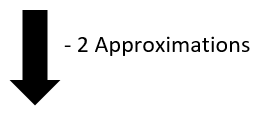
\includegraphics[width=4cm]{Arrow3.png}
	\end{figure}
	\vspace{-0.3cm}
	\begin{align*}
	&\frac{\partial \rho}{\partial t} + \nabla \cdot \left(\rho \mathbf{v}\right) = 0 \\
	&\frac{\partial \mathbf{v}}{\partial t} + \mathbf{v} \cdot \left(\nabla \mathbf{v}\right) + \gamma \mathbf{v} = - \frac{1}{m} \nabla \frac{\delta {F}[\rho]}{\delta \rho}
	\end{align*}
\end{frame}

\begin{frame}
	\frametitle{Summary}
	\begin{align*}
	\frac{d \mathbf{r}_i}{dt} &= \frac{\mathbf{p}_i}{m}\\
	\frac{d \mathbf{p}_i}{dt} &= - \gamma \mathbf{p}_i + \mathbf{X}_i(\mathbf{r}_i) + \mathbf{G}_i(t) \qquad \quad
	\end{align*}
		\vspace{-0.2cm}
	\begin{figure}
		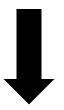
\includegraphics[width=0.4cm]{Arrow4.png}
	\end{figure}
	\vspace{-0.3cm}
	\begin{align*}
	\partial_t f^N = &- \frac{1}{m} \sum_{i=1}^N \mathbf{p}_i \cdot \nabla_{\mathbf{r}_i} f^N + \gamma \sum_{i = 1}^N \nabla_{\mathbf{p}_i}
	\cdot \mathbf{p}_i f^N - \sum_{i=1}^N \mathbf{X}_i \cdot \nabla_{\mathbf{p}_i}f^N + \gamma m k_BT \sum_{i=1}^N \nabla^2_{\mathbf{p}_i}f^N	
	\end{align*}
	\vspace{-0.2cm}
	\begin{figure}
		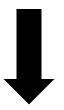
\includegraphics[width=0.4cm]{Arrow4.png}
	\end{figure}
	\vspace{-0.3cm}
	\begin{align*}
	&\frac{\partial \rho}{\partial t} + \nabla \cdot \left(\rho \mathbf{v}\right) = 0 \\
	&\frac{\partial \mathbf{v}}{\partial t} + \mathbf{v} \cdot \left(\nabla \mathbf{v}\right) + \gamma \mathbf{v} = - \frac{1}{m} \nabla \frac{\delta {F}[\rho]}{\delta \rho}
	\end{align*}
\end{frame}
\begin{frame}
	\centering
	\textbf{ \huge Part 3}
\end{frame}
\begin{frame}
	\frametitle{Part 3: Simplifications - The Overdamped Limit}
	We can take the overdamped limit when $\gamma$ is large.
	Then $\textcolor{red}{\frac{D \mathbf{v}}{D t} := \frac{\partial \mathbf{v}}{\partial t} + \mathbf{v} \cdot \left(\nabla \mathbf{v}\right) = 0}$
	\begin{align*}
	&\frac{\partial \rho}{\partial t} + \nabla \cdot \left(\rho \mathbf{v}\right) = 0 \\
	&\textcolor{red}{\frac{\partial \mathbf{v}}{\partial t} + \mathbf{v} \cdot \left(\nabla \mathbf{v}\right)} + \gamma \mathbf{v} = - \frac{1}{m}  \nabla \frac{\delta {F}[\rho]}{\delta \rho}
	\end{align*}
	So we get (32):
	\begin{align*}
	&\frac{\partial \rho}{\partial t} + \nabla \cdot \left(\rho \mathbf{v}\right) = 0 \\
	&\mathbf{v} = - \frac{1}{m \gamma} \nabla \frac{\delta F [\rho]}{\delta \rho}\textbf{}
	\end{align*}
	and finally get an overdamped equation in $\rho$ only (5):
	\begin{align*}
	&\frac{\partial \rho}{\partial t} -\frac{1}{m \gamma}  \nabla \cdot \left(\rho \nabla \frac{\delta {F}[\rho]}{\delta \rho}\textbf{}\right) = 0 
	\end{align*}
\end{frame}

\begin{frame}
	\frametitle{Part 3: Simplifications - The Diffusion Equation}
	From this overdamped equation:
	\begin{align*}
	&\frac{\partial \rho}{\partial t} -\frac{1}{m \gamma}  \nabla \cdot \textcolor{blue}{\left(\rho \nabla \frac{\delta {F}[\rho]}{\delta \rho}\right)} = 0 
	\end{align*}
	we can recover the diffusion equation! Choose
\begin{align*}
{F}[\rho] =  \int \rho(\mathbf{r}) (\log\rho(\mathbf{r}) -1)d \mathbf{r}
\end{align*}
then
\begin{align*}
\frac{\delta {F}[\rho]}{\delta \rho} &= \log \rho(\mathbf{r}), \qquad
\nabla \frac{\delta {F}[\rho]}{\delta \rho} = \nabla \log \rho(\mathbf{r}) = \frac{\nabla \rho}{\rho}, \qquad
\textcolor{blue}{\rho \nabla \frac{\delta {F}[\rho]}{\delta \rho} = \nabla \rho}. 
\end{align*}
and
\begin{align*}
&\frac{\partial \rho}{\partial t} -\frac{1}{m \gamma}  \nabla \cdot \textcolor{blue}{\left(\nabla \rho\right)} = 0  \quad \Rightarrow \quad \frac{\partial \rho}{\partial t} = \frac{1}{m \gamma} \nabla \cdot \left(\nabla \rho\right)  = \frac{1}{m \gamma}\Delta \rho = D_0 \Delta \rho
\end{align*}
	
\end{frame}
\begin{frame}
	\frametitle{Part 3: Simplifications - A Mean-Field Equation}
	From this overdamped equation:
	\begin{align*}
	&\frac{\partial \rho}{\partial t} -\frac{1}{m \gamma}  \nabla \cdot \textcolor{blue}{\left(\rho \nabla \frac{\delta {F}[\rho]}{\delta \rho}\right)} = 0 
	\end{align*}
	we can get a Mean Field Equation! Choose
	\begin{align*}
	\textcolor{blue}{\rho(\mathbf{r}_1,t) \frac{\delta {F}[\rho]}{\delta \rho}  =  \int \rho^{(2)}(\mathbf{r}_1, \mathbf{r_2},t) \nabla v_2(\mathbf{r}_1 - \mathbf{r}_2) d\mathbf{r}_2}
	\end{align*}
	then
	\begin{align*}
	&\frac{\partial \rho(\mathbf{r}_1,t)}{\partial t} -\frac{1}{m \gamma}  \nabla \cdot {\textcolor{blue}{\left(   \int \rho^{(2)}(\mathbf{r}_1, \mathbf{r_2},t) \nabla v_2(\mathbf{r}_1 - \mathbf{r}_2) d\mathbf{r}_2\right)}} = 0  
	\end{align*}
	
\end{frame}
\begin{frame}
	\frametitle{Part 3: Simplifications - A Mean-Field Equation}
	From this equation:
	\begin{align*}
	&\frac{\partial \rho}{\partial t} -\frac{1}{m \gamma}  \nabla \cdot {\left(\int \rho^{(2)}(\mathbf{r}_1, \mathbf{r_2},t) \nabla v_2(\mathbf{r}_1 - \mathbf{r}_2) d\mathbf{r}_2\right)} = 0  
	\end{align*}
	We make the mean field approximation:
	\begin{align*}
	 \rho^{(2)}(\mathbf{r}_1, \mathbf{r_2},t) \approxeq  \rho(\mathbf{r}_1,t) \rho(\mathbf{r_2},t)
	\end{align*}
	Then we get a mean-field equation:
	\begin{align*}
	&\frac{\partial \rho}{\partial t} -\frac{1}{m \gamma}  \nabla \cdot {\left(\int \rho(\mathbf{r}_1,t) \rho(\mathbf{r_2},t)\nabla v_2(\mathbf{r}_1 - \mathbf{r}_2) d\mathbf{r}_2\right)} = 0  
	\end{align*}
\end{frame}
\end{document}